% Chapter Template
% \doublespacing

\chapter{Introduction} % Main chapter title

\label{Chapter1} % Change X to a consecutive number; for referencing this chapter elsewhere, use \ref{ChapterX}

\lhead{Chapter I. \emph{Introduction}} % Change X to a consecutive number; this is for the header on each page - perhaps a shortened title

%----------------------------------------------------------------------------------------
%	SECTION 1
%----------------------------------------------------------------------------------------

\section{Rise of Unmanned Aerial Vehicles}
Unmanned aerial vehicles or UAVs have become ubiquitous in the past decade, both in research and industry. A myriad of applications involving UAVs in diverse fields has made them quite popular. Potential domestic  applications include Environmental monitoring and surveillance \cite{envmon}, traffic management \cite{trasur}, remote sensing \cite{remsen}, precision agriculture and farming \cite{preagr}, disaster management \cite{disman}, to name a few. The use of UAVs for defence purposes is only poised to grow in the next decade. It is not hard to see the appeal of UAVs in the defence sector with applications ranging from simple surveillance and reconnaissance missions to offensives like \textit{search and destroy} missions and targeted hits.

Much of the rise of this interest in UAVs can be attributed to associated advances in robotics, largely driven by the progress in robust and cheap sensors and communication technology. The emergence of scalable and extensible software architectures like the Robot Operating System(ROS), which enables easy integration of various subsystems further pushed the progress in these domains.

While early applications of UAVs were single UAV based, the focus is now shifting towards applications involving multiple UAVs, cooperatively completing tasks. There are several advantages of multi-UAV systems over single UAV systems. In certain applications like search and rescue missions, for instance, the use of multiple UAVs for surveying an area can significantly reduce the time taken to complete the task \cite{coosea}. As given by \cite{fanets}, other advantages of multi-UAV systems over single UAV systems include cost, scalability, survivability and speed.

Though UAV swarms have promising capabilities, they have quite a few challenges to overcome. Communication is one of the main hindrances to realize robust swarms of UAVs.

\section{The Challenge of Communications in UAV swarms}
While there is much literature regarding communication in UAV systems, \cite{fanets} and \cite{lavgupta} are two good survey articles regarding the current trends and issues in communication in UAV swarms. Besides pointing out the shifting interest towards multi UAV systems, due to their advantages over single UAV systems, they also identify the challenges in these systems, communication among the UAVs being the most notable one. 

Since the first applications were single UAV based, communication architecture in these systems was simple and straightforward. Often, there only needed to be a communication link between the UAV and the ground station. In some cases where the UAV has to cover a larger area, there could be multiple ground stations, and the UAV would have to communicate with the ground station near it. Even then, the overall architecture was pretty basic. As we noted earlier, there is a rapidly growing interest in realizing swarms of cooperative and collaborative UAVs, accomplishing complex tasks. Robust and reliable communication among the UAVs is an essential and critical component in enabling cooperative and collaborative behaviour in these UAV swarms.

While there is some interest in infrastructure based communication in UAVs, like using cellular infrastructure for UAVs \cite{celsur}, much of the research community considers enabling UAV communications in infrastructure less environments, more significant. These so called adhoc networks are important, for instance in disaster management scenarios where the existing infrastructure is damaged, or in military applications where there is no pre-existing infrastructure. The authors in \cite{lavgupta} try to identify several possible communication architectures for multi UAV networks.

\begin{figure}
	\centering
	\begin{subfigure}[b]{0.3\textwidth}
		\centering
		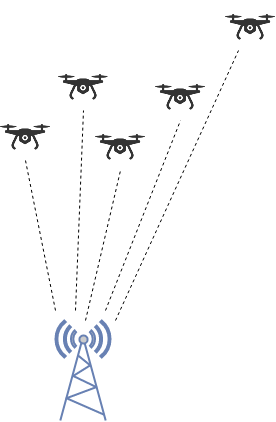
\includegraphics[scale=0.45]{Pictures/star.png}
		\caption{Star Configuration}
		\label{fig: starconf}
	\end{subfigure}
	\begin{subfigure}[b]{0.3\textwidth}
		\centering
		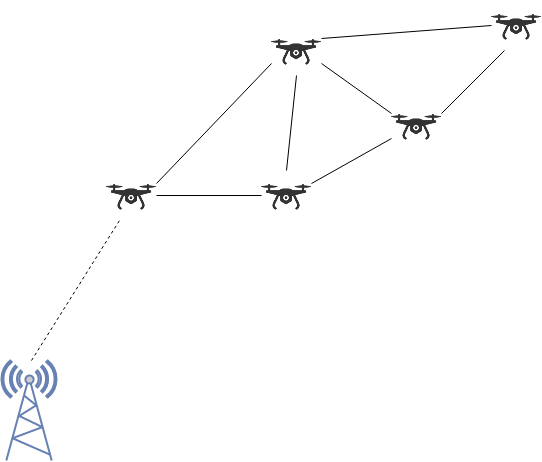
\includegraphics[scale=0.45]{Pictures/mesh.png}
		\caption{Mesh Configuration}
		\label{fig: meshconf}
	\end{subfigure}
	\caption{Possible network configurations for communications in UAVs}
	\label{fig: netconf}
\end{figure}

Figure \ref{fig: starconf} shows the star topology, where all the UAVs are connected to the ground station. In this configuration, the necessary communication among UAVs also needs to be routed through the ground station. Figure \ref{fig: meshconf} shows the mesh topology, where the UAVs communicate among themselves using an adhoc network, they themselves form. Typically, the ground station is also a part of the adhoc network. In the star configuration, since all the data has to be routed through the ground station, there would be higher latency and congestion in the network.

On top of that, if the UAVs are considerably far from the ground station, the network in star configuration may not provide reasonably high bandwidth for the communication among the UAVs. Moreover, if any of the UAVs loses its link to the ground, it cannot be accessible by any other UAVs, even if they are close. It is clear to see that the mesh configuration has a considerable advantage over the star configuration. Indeed, there is a consensus in the literature that realizing adhoc networks is the best solution for communication in multi UAV systems. There is a growing intereset in FANETs, the Flying Adhoc Networks. There is much literature in the filed and \cite{fanets} introduces and outlines the current and future trends in FANETs.

\begin{comment}
\section{FANETs, Flying Adhoc Networks}
While there were early attempts at different names for adhoc networks in UAVs like AUGNET \cite{augnet} and UAVNET \cite{uavnet}, the name FANET seems to be favoured. 

FANETs come under more general adhoc networks called MANETs(Mobile Adhoc Networks) and VANETs(Vehicular Adhoc Networks). MANET is the most general of the both and the oldest. There have been MANET protocols and standards defined to an extent.
\end{comment}

\section{Motivation and the Current Work}
With the advent of Internet of Things(IOT), there are now several communication standards which enable mesh networks like Bluetooth mesh networks \cite{blemesh}, Thread \cite{thread, thread2} and Zwave \cite{zwave}, where the last two protocols are based on the IEEE standard 802.15 \cite{meshsurvey}. Despite these, mesh networks which are based on the wifi, as standardized in IEEE 802.11s, better suit the needs of UAVs because of their high data rate and range.

While there are previous works which have used wifi based adhoc networks in UAVs like AUGNET \cite{augnet} and UAVNET \cite{uavnet}, they have several issues, not least of which is the range of the networks. Though the mesh networks enable reliable communication among the UAVs at an acceptable range, the link between the UAVs and the ground station is much more vulnerable. While the distance between the neighbouring UAVs can be kept relatively small, one cannot restrict the distance between the ground station and a UAV. A typical scenario would be that of a group of UAVs flying as a swarm far from the ground station. Even though the UAVs are in range and allow communication among themselves via the wifi mesh, the ground station at a larger distance can no longer be a part of the mesh. This is certainly a limiting factor in mesh networks for UAVs. This is one of the motivations for this work, in which we address this issue by using two different radio modules, a long range and a short range one(the wifi mesh). We propose a new architecture which blends short range and long range aspects of the communication. Note that the long range radios typically provide low bandwidth and are not suited for robust inter communication among the UAVs, demanded by many emerging distributed applications. This is not a concern in the case of the link between the UAVs and the ground station as long as, much data is not needed at the ground station, which is the case in autonomous applications, where much of the decision making happeds on board the UAV and ground station is merely used for monitoring.

Another aspect of motivation for this work is its integration with the Robot Operating System or ROS. ROS is a widely accepted software platform for research in robotics, which became popular as \textit{Linux for Robotics.} ROS, with its distributed and modular architecture, active development, collabarative environment and vibrant community has seen widespread adoption by individuals and organizations, across the board in robotics research. Thus the goal was to integrate our communication architecture into ROS, enabling development of distributed applications among UAVs without the need to worry about the underlying communication architecture.

\section{Organizaiton of the thesis}
We have introduced and motivated the problem of communication in UAV swarms in chapter \ref{Chapter1}. In chapter \ref{Chapter2}, we shall look at the development of the mesh architecutre. We shall look at the long range communication architecture in chapter \ref{Chapter3}. We shall look at some future work and  finally conclude this thesis with chapter \ref{Chapter4}.